%
%Paper for FC 2019
%Title: How to encourage cryptocurrency exchange to secure their system
%Authors: Shin'ichiro Matsuo, Yuta Takanashi, Pindar Wong, Eric Burger
%

\documentclass[english]{llncs}
\usepackage[T1]{fontenc}
\usepackage[latin9]{inputenc}
\usepackage[dvipdfmx]{graphicx}
\usepackage[title,toc,titletoc,header]{appendix}

\usepackage{babel}
\pagestyle{headings}

%\title{What is Cryptocurrency Exchange? - the reality and how to secure it}
%\title{Reality of less trust than expected to trustless financial system}
\title{Keep Cryptocurrency Exchanges Healthy: Lessons from Japan's Regulatory Experience with Mt. Gox and CoinCheck}

%\titlerunning{Reality of less trust than expected to trustless financial system}
%\author{
%Yuta Takanashi\inst{1,2}\and Shin'ichiro Matsuo \inst{1} \and Pindar Wong\inst{3} \and Eric Burger\inst{1} \and Masashi Sato\inst{4} \and Masaki Shimaoka\inst{4} \and Hirotaka Nakajima\inst{5}}
%\institute{Georgetown University
%\and Financial Services Agency
%\and VeriFi Ltd.
%\and SECOM Co., Ltd.
%\and  Mercari, Inc.}
%\date{\today}
\renewcommand{\baselinestretch}{0.98}
\begin{document}
\maketitle

\begin{abstract}
After the original publication of the Bitcoin paper~\cite{N08}, cryptocurrency exchanges emerged to connect the fiat currency world to the cryptocurrency world.
Although many users of cryptocurrency exchanges demonstrate confidence in this simple role for an exchange, recent security incidents suggest that a gap
%may exist
exists
between the perception of users and the reality.
% of the cryptocurrency exchange management.
%That is, what kinds of operations are conducted, what are the informational asset to be protected, and what kinds of security postures are required.
That is, operations, informational asset to be protected, and security postures should be clarified.
In this paper, we summarize the results of an investigation of 16 registered and 16
%quasi-registered
semi-registered
cryptocurrency exchanges by Japanese regulators, then analyze the reality of functionalities, implementation, and operations of
%real
cryptocurrency exchanges. Then,
from
%an information security management system (ISMS)
%standard
ISMS
point of view, we analyze relevant features of the blockchain protocol, cryptographic key management, system security, and operation, and clarify the required actions to secure the implementation and operation of cryptocurrency exchanges. We argue that the current activities in the IETF and ISO to develop
%a common standard
common document
%for securing
to secure
cryptocurrency exchanges would help industry as well as regulators to move forward towards establishing a healthy ecosystem.


{\bf Keywords:} Cryptocurrency exchange, Information security management, Standards
\end{abstract}

\section{Introduction}
%\paragraph{Background}
Eliminating the trusted third party in realizing network-based services is one of the biggest dreams in applied cryptography.
%cryptographic research.
% Hence this is the main subject in this world.  The main reason why we seek to eliminate the trusted party is, it is too difficult to realize expected trusted party. Such difficulties are caused by operator's mistakes, malicious activities, and collusion with other parties. Many cryptographic techniques like secret sharing scheme, threshold cryptography, and multi-party computation
%protocol are well studied to realize many network-based services without trusted parties.
%The sentence, ``An electronic payment system based on cryptographic proof instead of trust, allowing any two willing parties to transact directly with each other without the need for a trusted third party.'' is the explanation of Bitcoin - one of the most attractive cryptographic protocols - described in the original paper~\cite{N08}. Bitcoin is one of the most excellent cryptographic protocols which
%claimed to realize payment scheme among cryptographic protocols which try to eliminate the trusted party.

Despite this attractive claim of bitcoin,
%there
% is a
%are fundamental
%assumption
%assumptions
%in the claim. That is, it holds only when the payment is conducted by bitcoin, and no exchange to any other
%payment
%methods exists. Its ``without trusted third party'' claim realized by the distributed protocol is applicable only on the ledger of payment record for bitcoin.
%If we wish to exchange Bitcoin to other assets like fiat currency, the action of exchange is outside of what original paper claims. %That is, we need to assume some kinds of trust at a party which exchanges
%so-called
%trust-less cryptocurrency to other assets. Most people believe that cryptocurrencies are operated in the ``trust-less'' manner, as most cryptocurrency advertisement says. However, the cryptocurrency exchanges in real life are
%(hidden)
%hidden trusted parties.
%
throughout the history of trust-less cryptocurrency, there are many incidents have happened. In 2013, Mt. Gox lost many Bitcoin due to their careless operation and transaction malleability. In 2018, CoinCheck was hacked by a targeted attack and lost over 500M dollar equivalent NEM,
% which 700,000 customers deposited in their account at CoinCheck.
and Zaif also lost 50M dollar.
%There are many other examples of cryptocurrency incidents reported.
% from all over the world.
%Such incidents are caused by a misunderstanding of required trust in operating
%such
%a party.
% associated with trust-less cryptocurrency.
%When considering the amount of value that such companies deal with, these companies - implicitly assumed to be trusted - should be secure enough against any kinds of attacks including cyber attacks.
% and attacks on cryptography, key management.
%However, even now, such companies do not have enough expertise and human resources to secure their implementations and operations against such security concerns.
%
Usually, when we build an information system, we conduct design and implements of security mechanisms and operations, with aligning information security management system (ISMS)
%which is standardized in
%as
%the ISO/IEC 27000 series. The process includes threat modeling, risk analysis, and design and implementation of security %countermeasure and operations.
However, at this moment
there isn't any agreed unified security standard.
% for organizations and entities related to cryptocurrency and blockchain.
%Moreover, there is no standard software suite to build a cryptocurrency exchange.
%Hence, the design and implementation of each cryptocurrency exchanges vary among operators.  This situation makes operations challenging to secure the cryptocurrency exchange.

%Given this situation, we first need to figure out the reality of cryptocurrency exchanges, and then we need to proceed to implement existing ISMS process into implicitly trusted party associated with the trust-less ecosystem. We also need to reconsider the governance of such organization and entity. Above analysis and consideration helps to identify the required technologies, operations, and standards for cryptocurrency exchanges.
%\paragraph{Contributions}
The aim of this talk is giving a real status on the security of cryptocurrency exchange to consider future of uniformed security technology, management, governance, and standard.
Firstly, we will show the results of investigation and audit to 32 cryptocurrency exchanges in Japan, conducted by the Japanese Financial Services Agency, the governmental regulatory authority of Japan. The investigation and audit were conducted right after the incident at CoinCheck.
% (January 26, 2018). This includes analysis of the actual incidents, perspectives of investigation and results.
From this starting point, we give a detailed analysis of
%the difference between their advertisement and reality,
what levels of security and governance are implemented and what are missing.
Then we reconsider the governance and security management required to cryptocurrency exchange.
%, which
%including threat modeling of existing form of exchange. Then we show the required technology,
%and
%operations
%, and standard
%from the above analysis, as well as the recent progress of standardization.
%of blockchain and cryptocurrency exchange security
%in ISO TC307 and IETF.
%The construction of this paper is as follow. Section 2 describes the result of investigation and audit to 32 cryptocurrency exchanges. Then, we analyze the result in section 3. Section 4 discusses the desired governance and security management conclusions.
% from the above analysis.
%We also discuss future direction toward security standard of technologies and operations for cryptocurrency exchange and explain the current status of security documents in ISO and IETF.
%, which are also led by the author of this paper.
%In section 6, we conclude this research.

\section{Investigation and audit to 32 cryptocurrency exchanges}
\label{investigation}
\subsection{Security incidents and their history}
\label{subsec-incidents}
After Bitcoin was introduced in 2008, there have been many incidents happened at cryptocurrency exchange. Following are the summaries of major incidents happened in Japan.
%Table 1 shows the past major incidents which happened at cryptocurrency exchanges.
%Here, we describe the abstract of three major incidents and their source of problems.
%\begin{table}
%\begin{center}
%\caption{Major incidents at cryptocurrency exchanges}
%
%\begin{tabular}{|c|c| c | c |}\hline
%Name of Exchange & Dates & Amount of lost (at that time) & Abstract of incidents \\ \hline
%MyBitcoins & July 29, 2011 & 27,000 BTC (\$370,000) & disappear \\ \hline
%Linode & March 2012 & 46,703 BTC (\$200,000) & Web host hack\\ \hline
%Bitcoinica & March and May 2012 & 61,000 BTC &  Web host hack\\ \hline
%Bitfloor & September 2012 &24,000 BTC (\$250,000) & Server attack \\ \hline
%Mt. Gox & February 2014 & 850,000 BTC (\$473,000) & transaction malleability \\
%  &   &  &  and server hack\\ \hline
%Bitstamp & January 2015 & 19,00 BTC & Server attack \\ \hline
%Cryptsy Exchange & July 2016 &  11,325 BTC & Server attack  \\ \hline
%Bitfinex & August 2016&  119,756 BTC & Server attack  \\ \hline
%Gatecoin & 2016&  250 BTC, 185,000 ETC &  Attack on hot wallet\\ \hline
%Zaif & January 2018&  dollar &  \\ \hline
%NiceHash & December 2017 & 4,700 BTC &  Server attack \\ \hline
%CoinCheck & January 2018 & 580M dollar & Targeted attack \\ \hline
%BitHumb & June 2018 &  30M dollar  &  Server attack\\ \hline
%Monappy & September 2018 &  & Attack on hot wallet \\ \hline
%Zaif & September 2018 & 50M dollar & Attack on hot wallet \\ \hline
%\end{tabular}
%\label{table-incidents}
%\end{center}
%\end{table}

%Not all future work should be done to complete the table

\paragraph{Mt. Gox incident (2014):}

Mt. Gox was the world largest cryptocurrency exchange in 2014, which occupied about 70\% of bitcoin transaction.
The exchange did not segregate customers' assets from the exchange's asset.
The customers' assets were not recorded into Bitcoin blockchain
but recorded into some segregated ledger.
Thus, the attacker had a chance to attack the segregated
ledger instead of the attack on the blockchain and cryptographic keys itself.
The CEO of Mt. Gox claimed that the incident was caused by
transaction malleability of Bitcoin protocol.
By utilizing this vulnerability, the adversary
could convince the exchange modified transaction IDs.
This was one of factors of stealing bitcoins.% which were stored in the exchange.
Several experts pointed out that the loss was caused by this vulnerability,
but other significant factor of lost was internal malicious activities and
attack on segregated ledger from outside.



\paragraph{CoinCheck Incident (2018):}
In January 2018, CoinCheck, one of the biggest cryptocurrency exchange, but it was semi-registered to Japan Financial Service Agency (JFSA) was hacked and about 526,800,010 XEM was stolen. It was equivalent to 500M dollar. 260,000 customers of CoinCheck where victims.
This incident happened by the targeted attack as the first step. Adversary sent CoinCheck several emails to inject malware. As a result, the adversary succeeds to
intrude into the CoinCheck's network. The adversary could control computers remotely; then the adversary obtained a secret cryptographic key. After that, the adversary
sent XEM stored inside the CoinCheck's network outside within 30 minutes.
This indicates that all XEM are associated with one secret cryptographic key, and the amount of coins which each customer have is managed with a segregated ledger.
This was the same situation as the Mt. Gox incident.
The XEM stored in the hot wallet, that is the device that was connected to the internal network. Multi-signature, which is a general technique to divide signing privilege among
multiple persons, was not implemented. The main reason why CoinCheck did not implement was, the cryptographic algorithm and its parameter (elliptic curve) did not fit to
software/hardware of key management device. This implies, the kind of coin can affect the specification and operation of cryptocurrency exchange, but such
difficulties were not disclosed at that time.

\paragraph{Zaif Incident (2018):}
In September 2018, a hot wallet in Zaif was hacked and about 50M dollar equivalent Bitcoin and other cryptocurrencies were lost.
The specific problems of Zaif are it is registered cryptocurrency exchange under the current regulation. Moreover Zaif was
subject to administrative sanctions twice after the investigation described in this section. But, it did not
compliant these sanctions.

\subsection{Perspectives of investigations}
In May 2016, JFSA has amended Payment Service Act to ensure the trust of cryptocurrency users and AML/CFT, and has mandated cryptocurrency exchanges to register to JFSA and comply with legal requirements since April 2017.\footnote{JFSA has allowed companies which had already operated when the regulations was implemented to continue operation during the registration process. Thus registered exchanges and under-registration exchanges exisit as of September 2018.} In April 2017, JFSA also introduced Guidelines for administrative processes explaining how JFSA will supervise exchanges. In it, JFSA clarifies that 1) it will check each cryptocurrency if it is appropriate for exchanges to deal with from the view point of user protection and public interests, 2) it will check management's ability to ensure the operational adequacy including a) legal compliance, b) user protection, and c) risk management, and 3) foreign exchangers which provide services to people living in Japan need to register to JFSA~\cite{FSAGUIDELINE}.

After the CoinCheck incident, JFSA conducted monitoring on all the 32 companies and the on-site inspections of 7 registered and all the 16 under-registeration exchanges to check if they comply with the regulation. In so doing, JFSA clarifies that it reviews the business practices, the risks and compliance management, as well as the internal audit and corporate culture/governance, especially focusing on the perspectives including 1) the practice of assessment on the risk characteristics of the cryptocurrency a company deals with, 2) adequacy of risk management, 3) practice on anti-money laundering and anti-illicit activities, and 4) Practice on segregation of customers' assets

On the basis of the findings from the on-site inspection, JFSA issued business improvement orders and business suspension orders to those companies with problems. It also turned down the registration request from one company. Receiving these orders, 12 under-registration companies gave up registration.

\subsection{Results of investigation and audit}
On August 10, 2018, JFSA published an interim report of the results of the on-site inspection and the monitoring with the aim of helping cryptocurrency exchanges to improve their business practices and regulatory compliance~\cite{FSAREPORT}. In section 2 of the report, JFSA shows numbers related to exchanges\footnote{Fig 1 to 3 and Fig 4 to 6 in the following shown in Page 4 and Page 5 of the JFSA's report respectively.}. Fig 1 shows the number of total assets of 13 registered and four under-registration exchanges in the last business year and Fig 2 shows the amount in the latest business year.
Fig 3 shows the change in the amount of total asset in one business year, which growth reaches on average 553\%. The report explains the massive increase of the total asset was caused by the hike in the exchange rate of the cryptocurrency against fiat currency since fall in 2017. Fig 4 shows the number of employees of all exchanges and Fig 5 shows customers' assets they manage. Based on these numbers, the report calculated the amount of customers' assets that one employee manages shown in Fig 6. JFSA point out by citing this number that very few people manage the huge amount of customers' assets; on average, one person manages \$30 million. %To give a sense of scale, this number is larger than \$16 million, which is the amount of deposit that one employee manages at MUFG, the largest Japanese financial group\cite{MUFG}.
JFSA explains that the establishment of the internal management was too slow to keep up with the rapid business expansion and management lacks awareness of the risks associated with the custody service managing the huge amount of customers' assets.

JFSA shows findings within the business practices, the risk and compliance management, and the internal audit and corporate culture/governance as summarized in the following.

\begin{center}
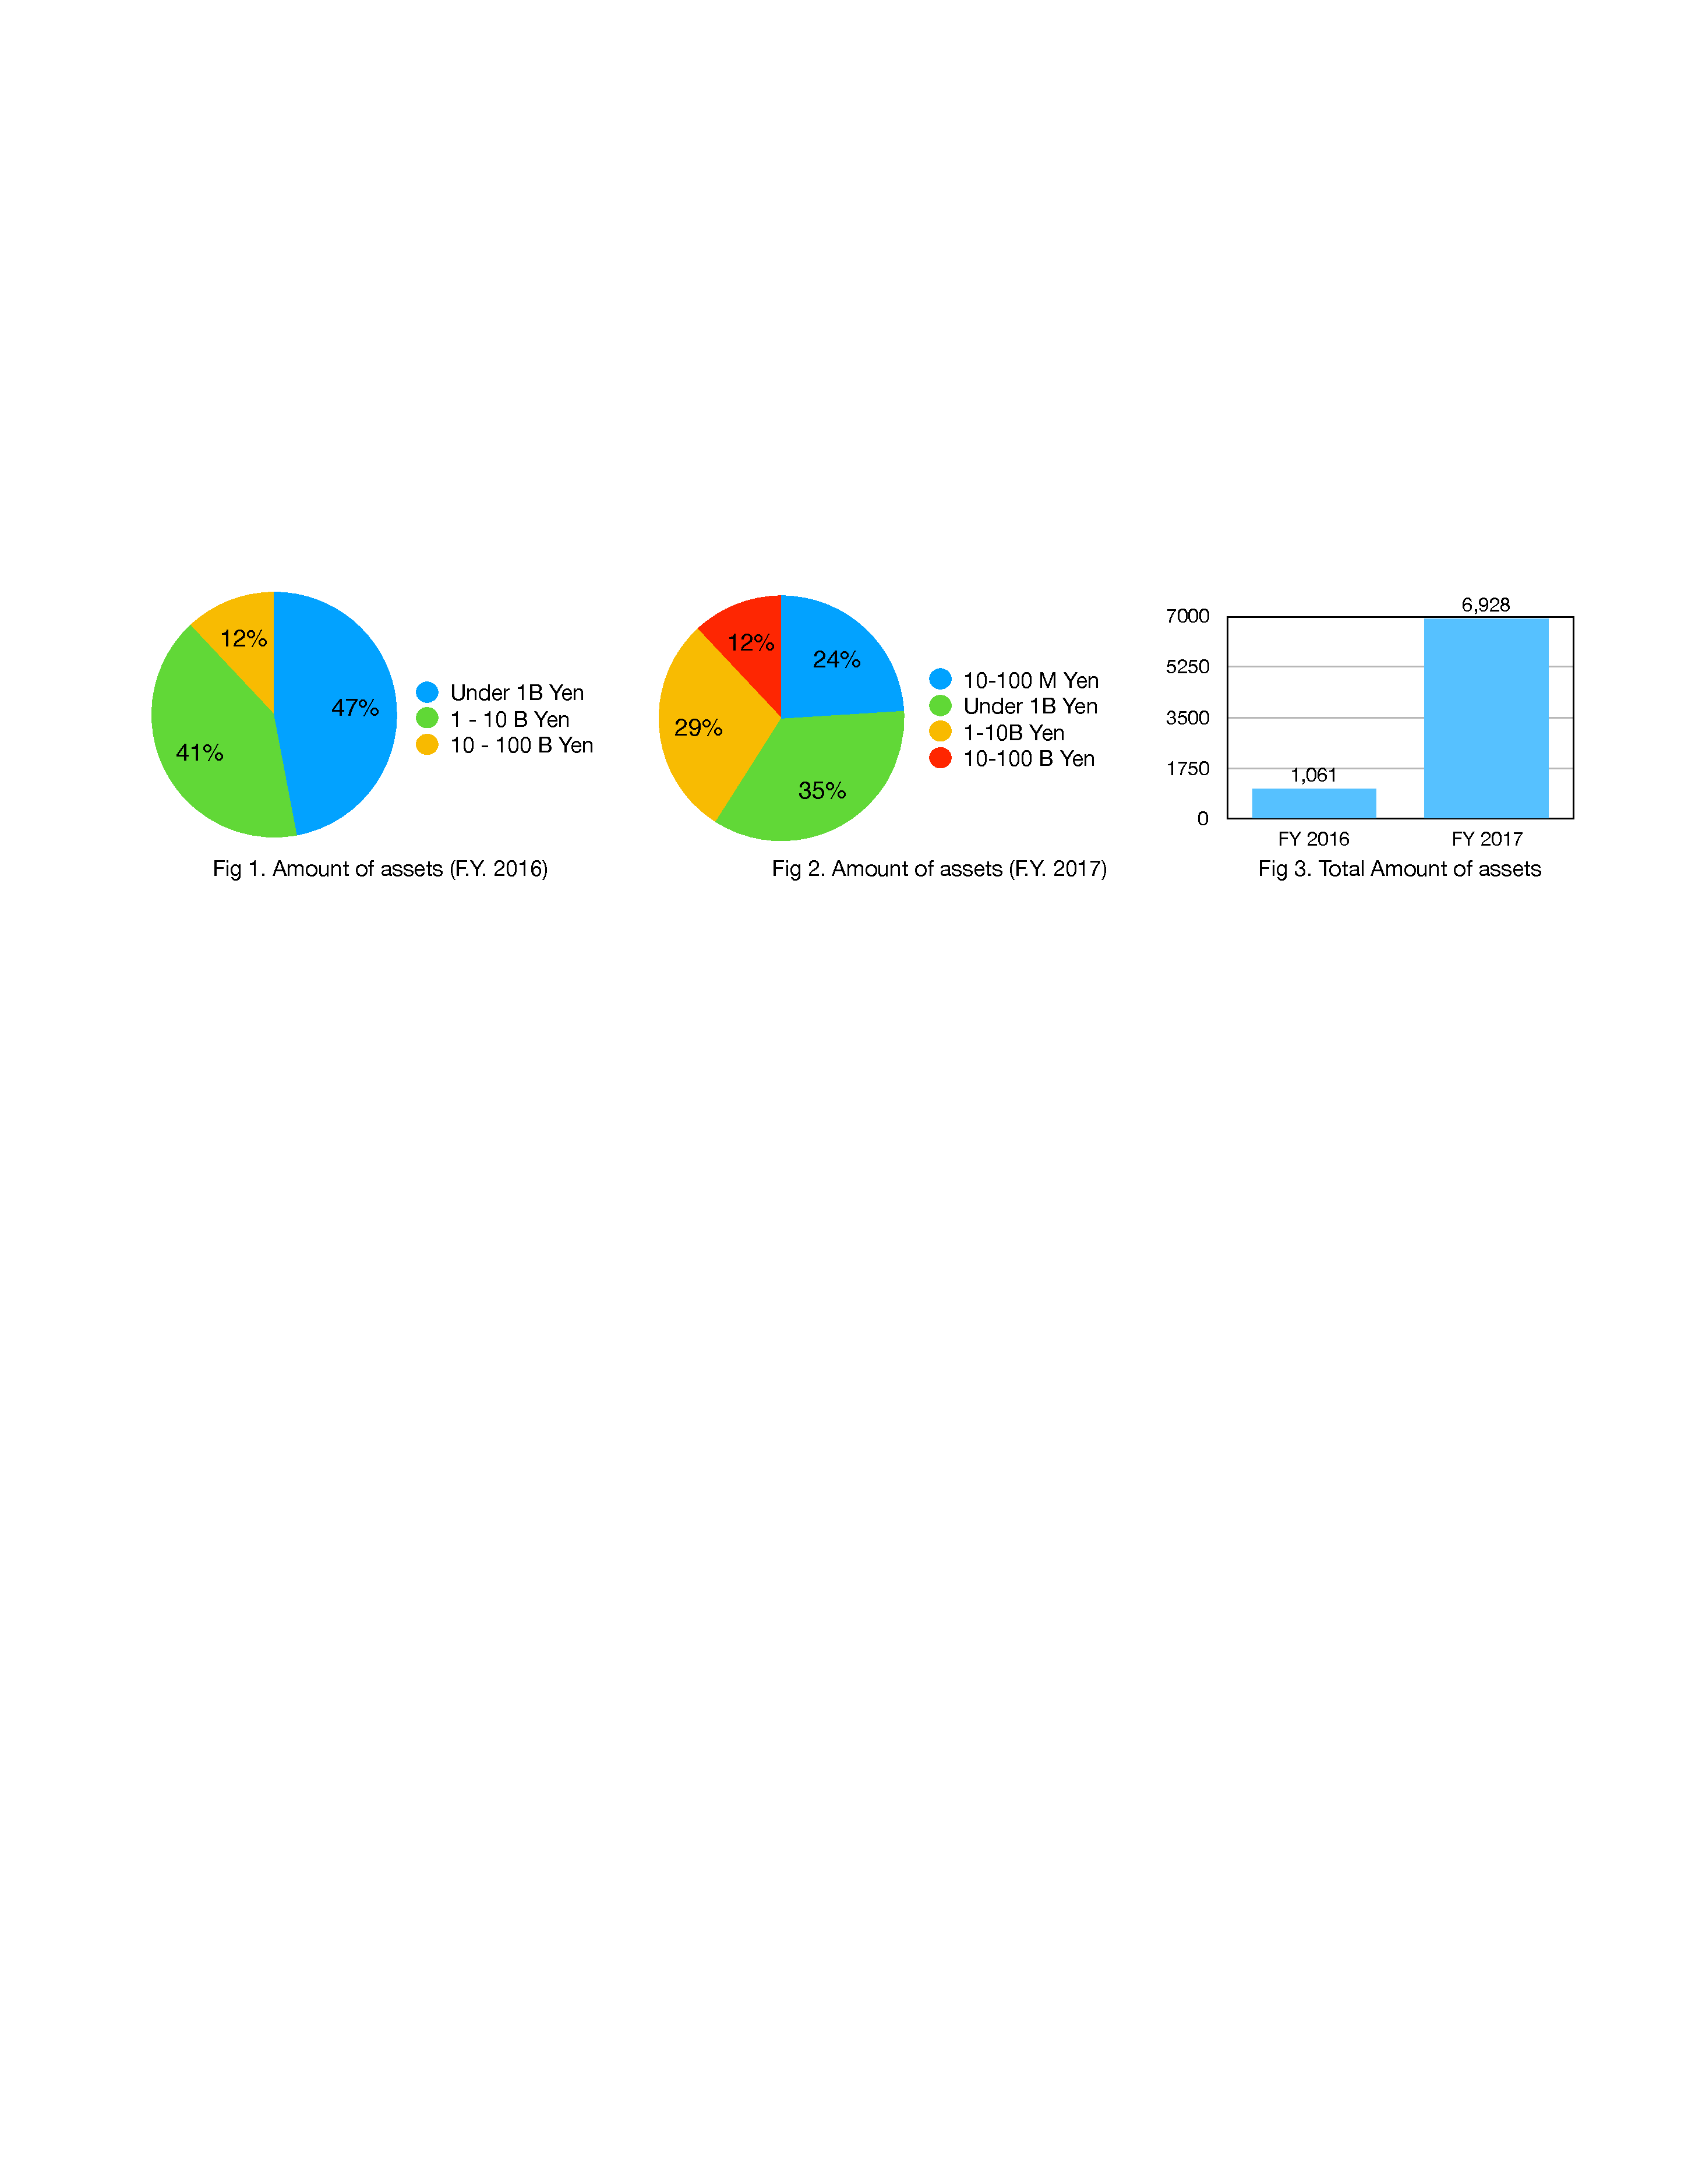
\includegraphics[width=9cm,pagebox=cropbox,clip]{fig1.pdf}
\end{center}

\begin{center}
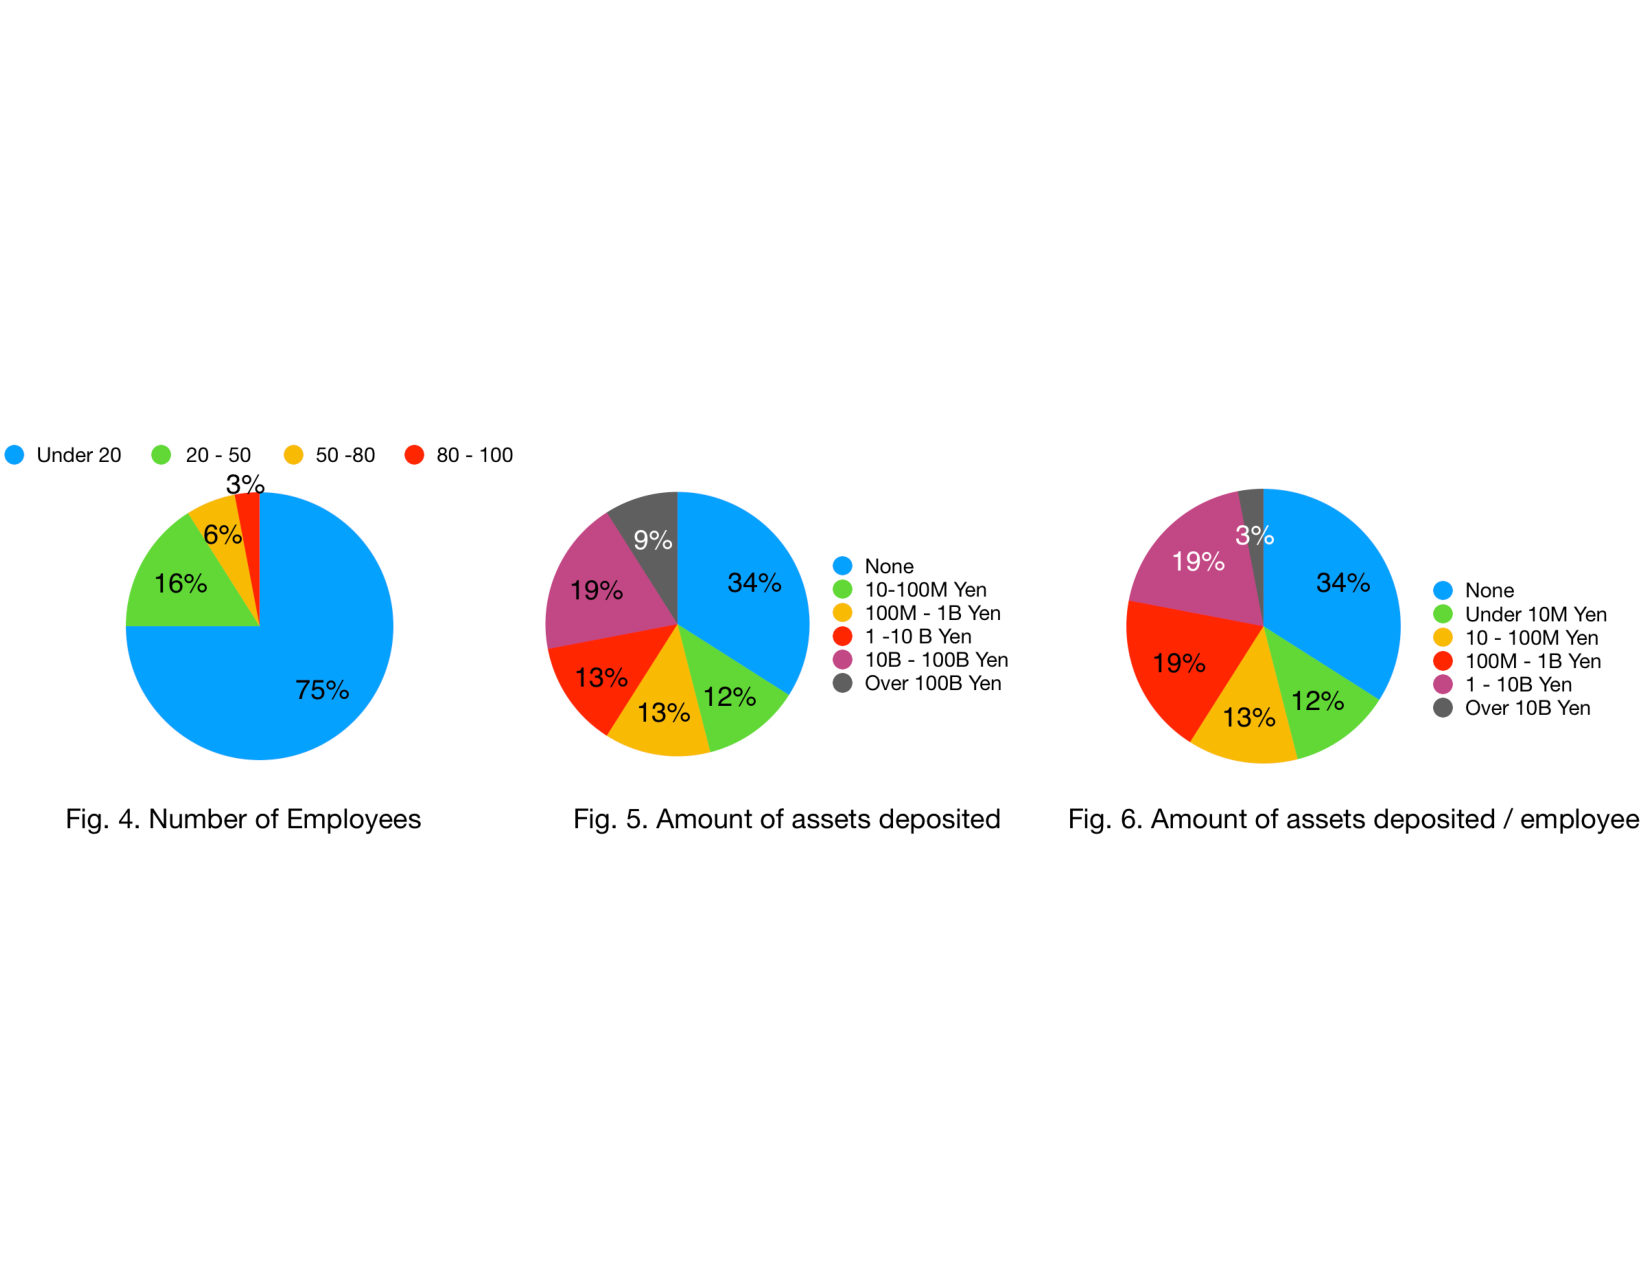
\includegraphics[width=9cm,pagebox=cropbox,clip]{fig2.pdf}
\end{center}

\subsubsection{Frontline: The business practices}
The report points out the issues around 1) selection process of cryptocurrency to deals with, 2) inappropriate distribution of cryptocurrency and 3) advertisement.
More concretely, the report explains that many\footnote{"Many" in this section means JFSA found similar issues in 8 or more exchanges.} exchanges lack business practices to assess risks associated with each cryptocurrency while they focus only on customer convenience and the profitability. And several\footnote{"Several" in this section means JFSA found similar issues in 2 to 7 exchanges.} exchanges lack internal rules that define investment limits and criteria for solicitation and transaction based on the `'principle of suitability' concerning customers' characteristics. The report even points out a case of price manipulation. There also found cases where advertisements of exchanges could mislead users.
%there is a case where an exchange does not have the internal review process of the contents of the advertisement. With regard to the advertisement itself, an exchange used TV advertisement on which famous celebrity calls the name of the certain cryptocurrency to encourage customers to buy it while explains risks only in few seconds. In another case, an advertisement shows a particular discount period and investment profitability that customers cannot verify.

\subsubsection{Second line: The risk and compliance management}
The report points out the issues around 1) AML/CFT, 2) segregation of customers' assets, 3) system risk management, 4) customer protection, 5) third party delegation.

For AML/CFT, several exchanges lack enough experts who can provide appropriate advice to frontline staff regarding risk managment. Thus many exchanges fail to comply with the regulation that requires multi-layer countermeasures for AML/CFT such as the establishment of internal guidelines, conducting customer due diligence, and monitoring of suspicious activities. The report shows a case where an exchange allows an organized crime group member to continue transaction for a while after the exchange realized that the customer is a member the group.
%In addition, there are issues around practices as well. For example, many exchanges fail to comply with the regulation that requires them to confirm customers' characteristics and purpose of the transaction as well as conduct pre-examination to exclude transactions with the anti-social group. There are cases of lack of appropriate guidelines regarding checking process of impersonation, and an exchange lacks monitoring process and system to detect suspicious activities.

For segregation of customers' assets, JFSA explains that several exchanges manage cryptocurrency in the hot (online) wallet, fail to reconcile on the daily basis between account balance within their server and that on the blockchain, and lack an ex-post verification process of reconciliation. Several exchanges also combine customers' assets and their own assets in order to keep the amount on the blockchain larger than the account balance within internal server. There is a case where an exchange even does not segregate customers' assets at all for some cryptocurrency. Yet another exchange, even when it recognizes that the account balance of internal server becomes below the balance on the blockchain, neither appropriately identify the cause nor address it. The report also points out the issues related to management of fiat currency in a similar manner. Furthermore, JFSA found that several exchanges fail to follow regulatory requirements on bookkeeping and an exchange even diverts money to other purposes.
%In addition, JFSA points out the issue around management of fiat currency. For example, several exchanges fail to reconcile between bank account balance for customers' assets and account balance on their own server.  Yet another exchange fails to find out the cause of the frequent incident that the customers' bank account balance becomes below the balance on their own server. Furthermore, JFSA found issues around bookkeeping. For example, several exchanges create general ledger only and fail to keep books on daily transactions, the ledger of their own account, and the ledger of customers' account, all of which are required by regulation.

For systemic risk management, JFSA shows that many exchanges lack human resources and training to manage the information system and fail to establish a contingency plan based on the risk scenario on cyber attacks. An exchange even issues new crypto assets without conducting a security evaluation of the underlining technology. JFSA also points out problems on authority management and countermeasures toward system troubles. For instance, within several exchanges, the same person develops and operates the system, and an exchange also fails to impose appropriate restrictions on holders of administrative IDs. Lack of record keeping and efforts to address the root cause of system troubles are also pointed out. In addition, lack of awareness of system limitation caused over capacityof of trading volume in an exchange.

For customer protection, the report mentions problems related to crypto assets issuance. There are several cases found in individual exchanges such as %lack of explanation about the financial situation and business model of the issuing exchange to customers,
failure to keep promise that the money raised is invested in new businesses, lack of clear understanding on accounting practices for cryptocurrency issuance, failure to disclose any unfair treatment including the huge discounts for insiders or realized differences between reality and the white paper. %and the huge bonus to management of the exchange for sale of the cryptocurrency.
JFSA also found issues that several exchanges fail to establish customer information management guidelines, %fail to conduct the training program on these matters, fail
lack access control on customer information and fail to address customer complaimnts in an appropriate way%, and allow anyone in the company and third-party contractor to access to it or even bring out from the company
.
%Several exchanges fail to either keep records of the customer complains or improve the business practice based on the complaints. They just ignore them or randomly address them case by case basis.
The report also shows examples where exchanges fail to conduct the assessment on volatility and trading volume of the cryptocurrency to decide loss-cut or set leverage limitation of margin trading.

For third-party outsourcing, the report explains several individual cases. For example, an exchange neither conduct the assessment of third-party contractor nor establish a formal outsourcing contract. %For another example, an exchange does not manage third-party contractor and fails to check the situation of outsourcing from the third party contractor. Another exchange does not request a third-party system developer to address issues related to system troubles.
Another exchange using cloud service fails to establish an outsourcing contract with its provider because of the lack of awareness that the cloud server is the third party to manage.

\subsubsection{Third line: The internal audit}
The report reveals that there are no internal audit or the internal audit is not based on the risk assessment within several exchanges. In many exchanges, there are not enough experts in internal audit implementation regarding AML/CFT and system risk management. For example, many exchanges fail to conduct the internal audit% or establish the plan for internal audit
because only one person who has another position is assigned to the position in charge of internal audit. %For other examples, several exchanges fail to conduct it based on the risk assessment or to conduct the audit on the third party contractor.
Furthermore, in an exchange, a person who is in charge of internal audit reports no problem even though the person, in fact, did not verify it.

\subsubsection{Corporate culture and governance}
The reports point out that exchanges prioritize profit making and lack culture of compliance and customer protection and internal management. For example. JFSA found that many exchanges fail to hire enough staff and improve IT system to support the expansion of the business. There is a case where management meeting focuses solely on expansion and advertisement but not on internal management. In an exchange, major shareholders and the management are not separated and management prioritizes profit of these shareholders.

Even though exchanges are in essence financial institutions, engineers who lack expertise in financial business manage the company. From the first point, many exchanges even lack awareness that they are financial institution dealing with huge amount of customers' assets% and fail to discuss how to mitigate risks associated with their business in the board meeting. The report also mentions that many exchanges fail to disclose their business and financial situation to customers in an easy-to-understand manner.

The weak management by the company's Board of Directors is also an issue. It is often the case that the CEO has too much power and the Board and internal audit fail to check the management. For example, several exchanges fail to keep the record of the Board meeting and the Board members are not well informed to play an appropriate role. For another example, the Board members fail to check if the money raised by token issuance is used as promised or check if the external auditor has enough knowledge and experience to conduct the appropriate audit.

\section{Analysis of the reality of ``Cryptocurrency Exchanges''}
%\subsection{How cryptocurrency exchanges introduce themselves and general persons recognize it}
%\label{perception_gap}
%TV CM, Okuri-bito, etc.

\subsection{Trends of the shortage of governance and security management}
% During JFSA, Japanese governmaenal regulation authority,  did audit and investigation, it issues administrative penalties to cryptocurrency exchanges with problems.
After the CoinCheck incident, JFSA issues 20 administrative penalties to 17 cryptocurrency exchanges.
Each release for the administrative penalty explains problems to be fixed. There are 22 kinds of problems are explained. There are 6 major problems and which problems are applicable to each cryptocurrency exchange.
% These 6 problems are those which over 25 \% of cryptocurrency exchange was requested to fix them.
They are Corporate management issue, system risk issue, anti-money laundering, segregation of customers' asset, customer protection and
consideration to deal with new cryptocurrencies.
% \begin{table}
% \begin{center}
% \caption{Major problems which each cryptocurrency exchange was requested to fix}
% \begin{tabular}{|c|c|c|c|c|c|c|c|c|c|c|c|c|c|c|c|c|c|c|}\hline
% Problems & (1) & (2) & (3)& (4) & (5) & (6)& (7) & (8) & (9)& (10) & (11) & (12)& (13) & (14) & (15)& (16) & (17)  \\ \hline
% Management & x & x &  & x & x & x & x &  & x &  & x & x &  & x &  & x &  x \\ \hline
% System Risk & x & x & x & x & x & x & x &  & x & x & x & x & x & x & x & x & x   \\ \hline
% AML & x & x & & x & x & x & x &  & x & x & x & x & x & x & x & x & x  \\ \hline
% Segregation & x &  & & x &  & x & x &  & x &  &  & x & x & x & x & x & x   \\ \hline
% Customer  & x &  & & x & x &  &  & x & & x & x & &  &  & & x &    \\ \hline
% New coin & x &  & & x &  & x &  &  & x &  &  & x &  &  & & x &    \\ \hline
% \end{tabular}
% \label{incidents}
% \end{center}
% \end{table}
% From this table, the first important result is that most of all
% cryptocurrency exchanges which were penalized, did not have qualified corporate management, system risk management and
% systems and operations for anti money laundering. This indicates there is no common understandings
% on the implementation and operations for financial services. The lack of management of system risks
% is indicates that such cryptocurrency exchanges do not have enough number of qualified system designers,
% engineers and operators. As we described in 2.1, most of incidents were caused by attacks from outside,
% and the amount of assets should incentivize the attackers to mount actual attacks. Thus,
% each cryptocurrency exchange should hire a group of experienced security experts. However, the reality
% is not the case.
%
% AML is the main issue from the regulatory authority point of view. However, most of all penalized
% cryptocurrency exchanges did not have enough operational capability in this. That is,
% such cryptocurrency exchanges did not hire such experts and hence they were not qualified as
% financial institutions.
Though corporate management and AML are the most crotical issues,
 the other things to be noted is the segregation of customers' asset.
%This is a quite fundamental operation
% as a financial institution, but over 50 \% of penalized cryptocurrency exchanges manage
% customers' assets with the institutional assets, private assets, or assets of multiple customers co-mingled.

\subsection{Functionalities which real cryptocurrency exchanges have}

%As described in~\ref{perception_gap}, t
There are many perception gaps between what user of cryptocurrency exchange think and real cryptocurrency exchange.
% From the word of ``Exchange,'' a general person think the task of the cryptocurrency exchange is matching selling orders to buying order
% like a general stock exchange.
%However,
A user has an account at the cryptocurrency exchange, then deposit some amount of money to the account. This implies the cryptocurrency exchange has similar functionality as a bank. Moreover, most cryptocurrency exchanges keep a (private) signing key of each user inside their server. This means such cryptocurrency exchanges have a functionality of custodian.
%By the investigation,
% described in \ref{investigation}
Some cryptocurrency exchanges do not record transfer of cryptocurrency into
the original blockchain.
%, but manage another database (hopefully some blockchain system) as a ledger inside the exchange.
In such case, cryptocurrency is ``sold'' in exchange of customer's money, but nothing is sold and the customer buys something
without the existence of the cryptocurrency.
In some case, cryptocurrency is sold by the exchange itself with some information as it seems matched with some order.
%However,
%the suggested price is shown by the exchange, and the transaction is conducted by price asked. In this case, the customer thinks
%he transaction is conducted by the result of matching over market,  but the reality is simple purchasing.
In th3se cases, the ``exchange.''
is not true exchange, but a currency shop.
There is an essential reason why an average customer deposits the private signing key to the cryptocurrency exchange is,
it is not easy to securely manage the private cryptographic key for such an average person.

% From above all, the functionality of cryptocurrency exchange is apparently beyond the ``exchange'', and in some case, it is
% a simple shop, and in the worst case, this might be selling nothing in exchange of real money.

\subsection{Shortage of security consideration}
From the analysis of functionalities described in the previous subsection, most of the existing cryptocurrency exchanges
have more functionalities than any one of the stock exchange, bank, custodian, and shop.
% Thus, the cryptocurrency exchange needs to manage security risks according to all the functionality it has.
% Hence, the security consideration should be the sum of security management for each function and more.
% With considering the amount of values each cryptocurrency exchange deals with, it should be a big target of cyber attacks.
% Such cyber attacks cause most of past incidents described in 2.1. Thus, each cryptocurrency exchange should be
% tolerant to global scale cyber attacks.

However, unfortunately, most cryptocurrency exchanges are startup companies. Thus, they do not have enough
capability to hire enough experts to design, implement and operate secure cryptocurrency exchange. The number of
such qualified experts is quite limited, thus attracting the sufficient number of qualified experts is not entirely a matter of money.
As a result, most cryptocurrency exchanges are not designed by general security management methodology for infrastructure.
They include not only cryptography but for security for the entire system, like protocol, authentication and access control, authorization,
network security, implementation and certification, key management, and operation.
However, such system-level security consideration was omitted.
For example, the early stage discussion right after the CoinCheck incident was a treatment of cold wallet, which is only a part of security management.

% \subsection{Issues which are common to the financial industry and specific to cryptocurrency exchange}
%
% Most of the issues
% % described in section \ref{investigation}
% are common to the financial industry. However, the rest is specific to cryptocurrency exchange.
% %Among six significant problems
% % described in 2.4,
% %corporate management and customer protection is common to the financial industry, and there are no specific matters to
% %cryptocurrency exchange. %Here, we describe issues specific to cryptocurrency exchange.
% %System risk is, of course, common to the financial industry, but
% The design and security management of
% information system depends on each specific business conditions. For example, key management is
% one of the biggest issues in the application of cryptography. Given the real world business of cryptocurrency
% exchange, many customers deposit their private cryptographic keys. The key management lifecycle is different
% from ordinary Public Key infrastructure (PKI).
% Informational assets, attack surfaces, threats, and risks
% vary due to each business environment. We will analyze the security management of
% cryptocurrency exchanges in section 4.
% AML is also a common issue for all financial business, but anonymous cryptocurrency causes
% many difficulties than ordinary financial services. In the case of CoinCheck incident,
% the stolen NEM coin could not be actually traced. Currently, cryptocurrency exchange is one of few targets of regulation, because it is the connecting point between cryptocurrency and real-world economy. With current regulation which fits FATF recommendation, most of all cryptocurrency exchange conducts verification of identity. Introduction of Decentralized Exchange (DEX) will eliminate the point of regulation. Thus it
% should increase this difficulty.
% % Dealing with a new coin is a new issue for cryptocurrency exchange. New cryptocurrency should be evaluated
% % on its characteristics and technical reliability.

\subsection{Discussion on key management}

% Segregation of customers' asset has another discussion issue.
% In the case of CoinCheck incident, all assets deposited at CoinCheck are managed by using one cryptographic key pair (address), and this is the reason
% why the entire customer assets were stolen in a short time period.
In the CoinCheck incident, the stolen cryptocurrency was NEM, of which the underlying consensus mechanism is based on Proof-of-Stake (PoS).
There are many reasons including transaction throughput, to manage the assets of many customers by using one key.
% It is not clear that this was the reason why CoinCheck managed the all assets by using one address. However, i
In general, PoS type cryptocurrency may
give cryptocurrency exchange terrible incentive to manage all assets with one key, because the cryptocurrency exchange can gain mining (or similar) reward by utilizing the vast amount of customer's cryptocurrency.  As a result, cryptocurrency exchange produces a new single point of failure, and it is
things should be avoided from the security point of views. Of course, this type of operation is out of the scope of cryptocurrency, but we need to care about the possibility to
happen this kind of things.
Each consensus mechanism has pros. and cons. generally. However, this is one issue of the downside of PoS type cryptocurrency, and we need to have
clear operation policy for PoS type cryptocurrency.

\section{Reconsidering governance and security management}
\subsection{Threat modeling and security requirements}
\setcounter{figure}{2}

In parallel to the investigation by JFSA, we conducted making a document on security management of cryptocurrency exchange right after the CoinCheck incident.
% One of the author of this paper is a member of this group.
%The purpose of the study is collecting practices of constructing and operating the cryptocurrency exchange.
%
Even now, there is no standardized architecture and implementation of software/hardware for cryptocurrency exchange. Therefore, we cannot edit one standard document toward secure implementation and operation of cryptocurrency exchange. The group gathered information of real cryptocurrency exchanges from their engineers, then create a model of cryptocurrency exchange system. Fig.~\ref{fig_system_model}. shows an example of system model of cryptocurrency exchange.

% \begin{figure}
%  \begin{center}
%   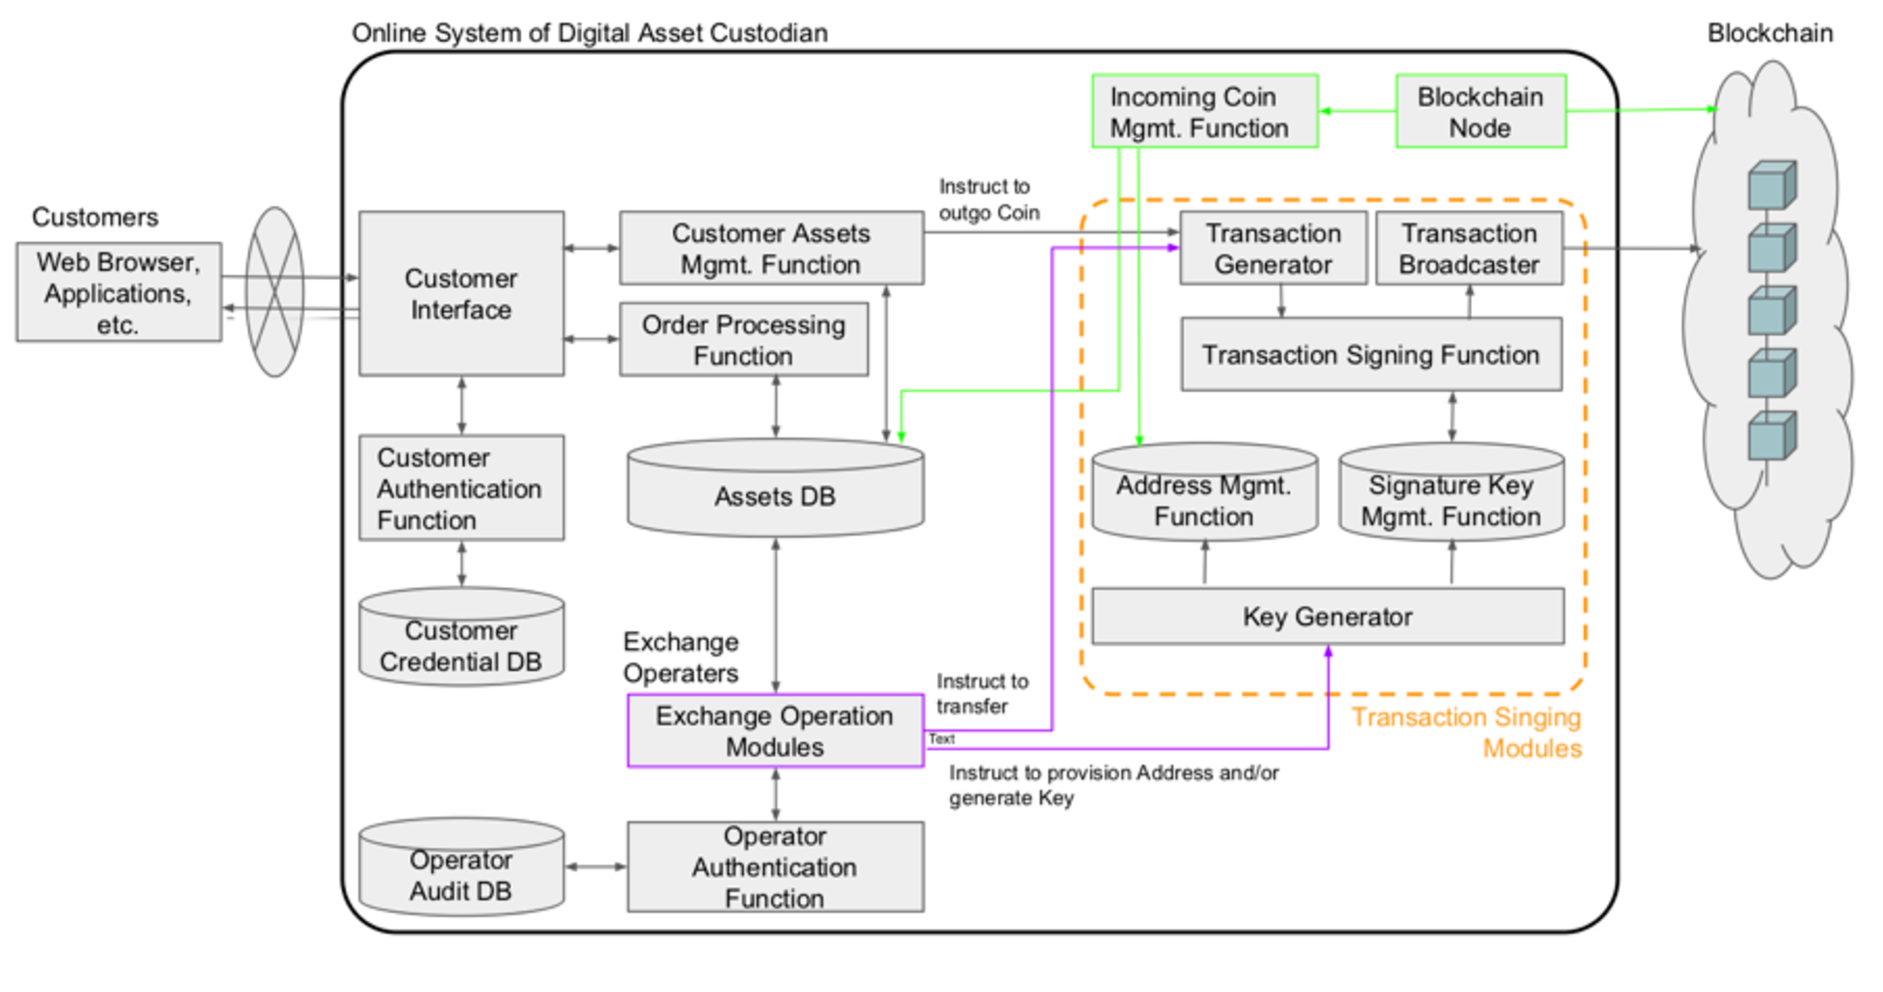
\includegraphics[width=8cm,pagebox=cropbox,clip]{system_model.pdf}
%   \caption{System model of cryptocurrency exchange}
%   \label{fig_system_model}
%  \end{center}
% \end{figure}
%
% \begin{figure}
%  \begin{center}
%   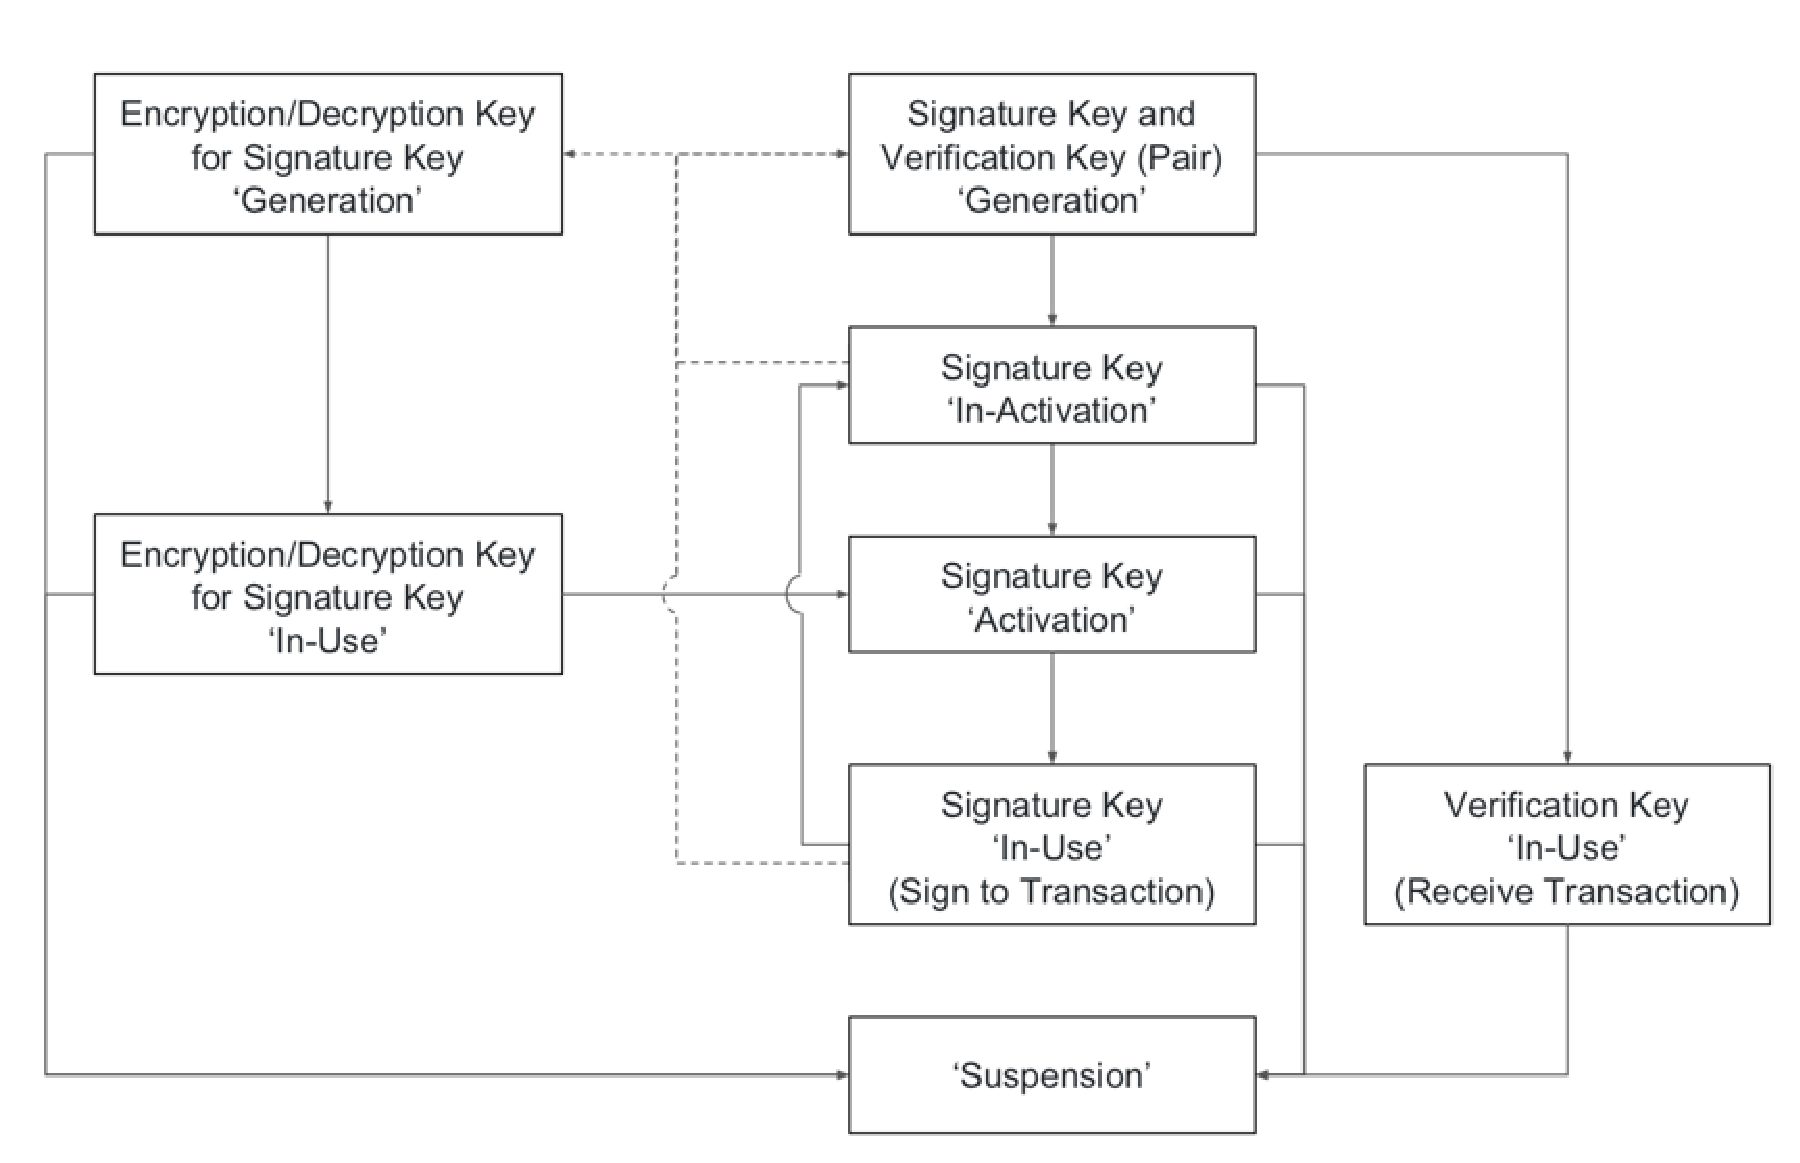
\includegraphics[width=8cm,pagebox=cropbox,clip]{key_lifecycle.pdf}
%   \caption{Key life-cycle at cryptocurrency exchange}
%   \label{key_lifecycle}
%  \end{center}
% \end{figure}

\begin{figure}[htbp]
  \begin{tabular}{cc}
    \begin{minipage}{0.5\hsize}
      \begin{center}
        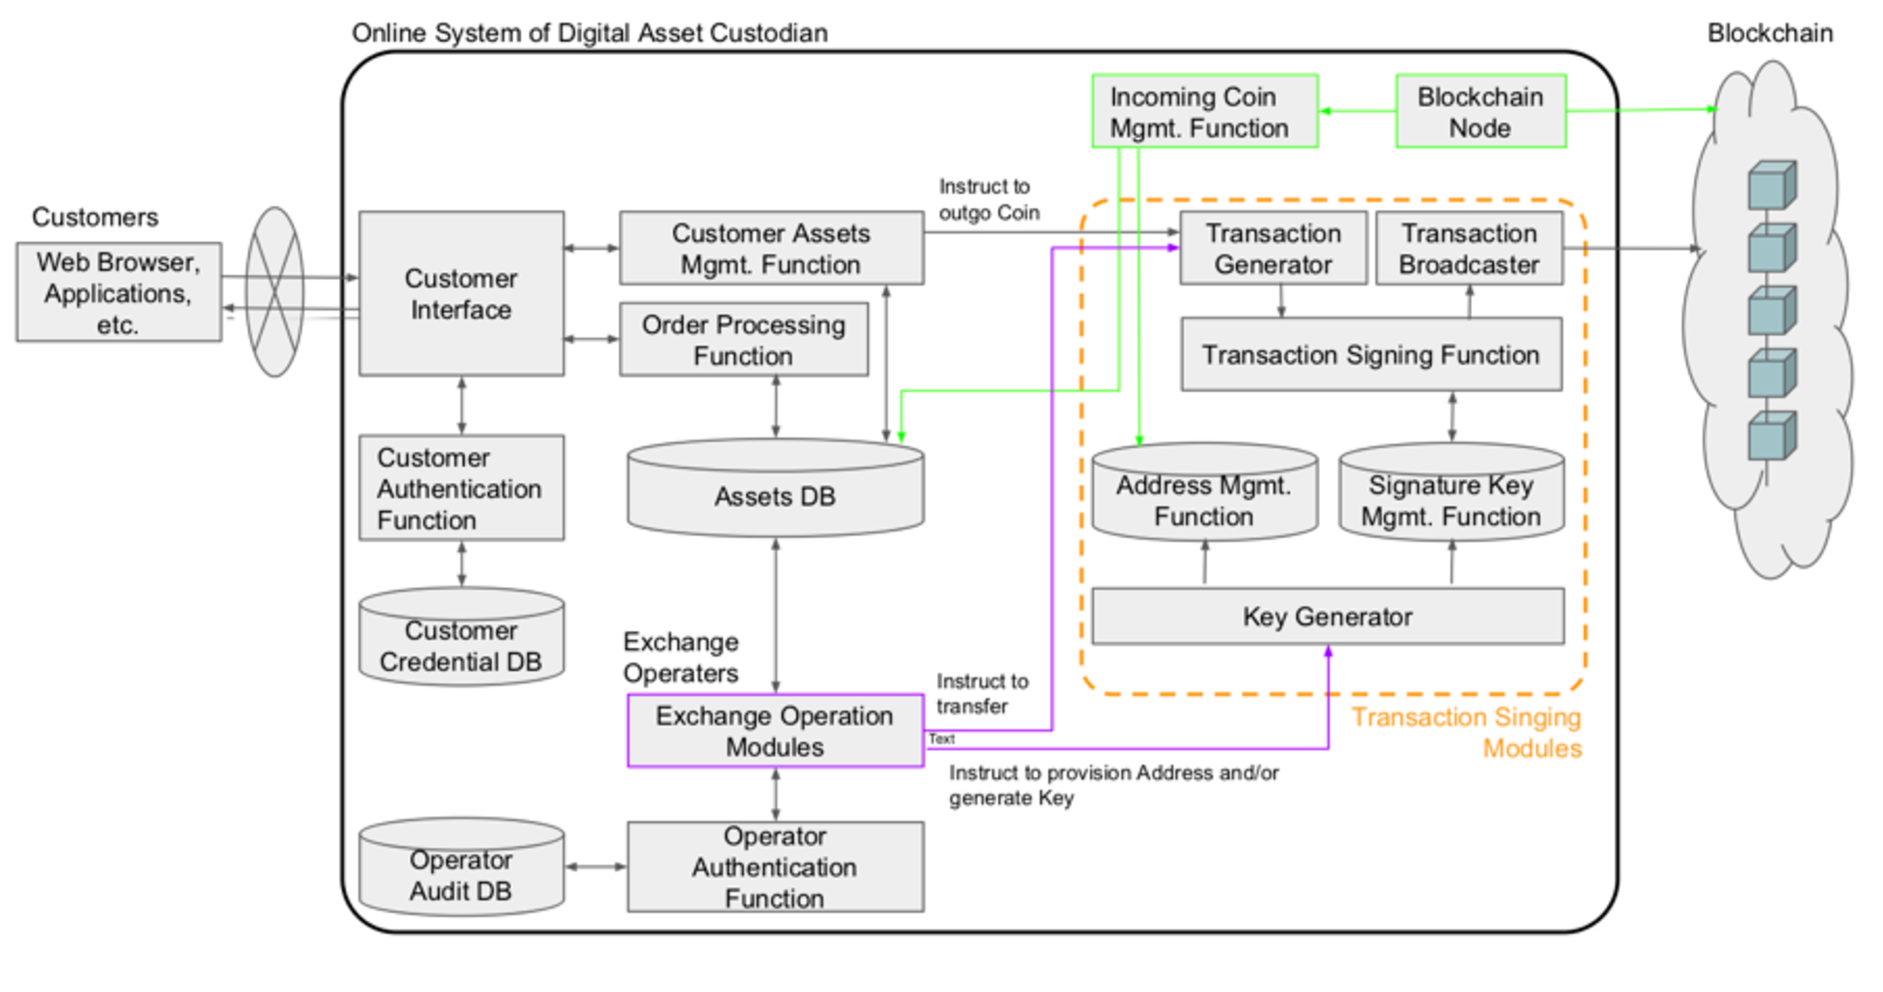
\includegraphics[width=6.5cm,pagebox=cropbox,clip]{system_model.pdf}
        \caption{System model of cryptocurrency exchange}
        \label{fig_system_model}
      \end{center}
    \end{minipage}
    \begin{minipage}{0.5\hsize}
      \begin{center}
        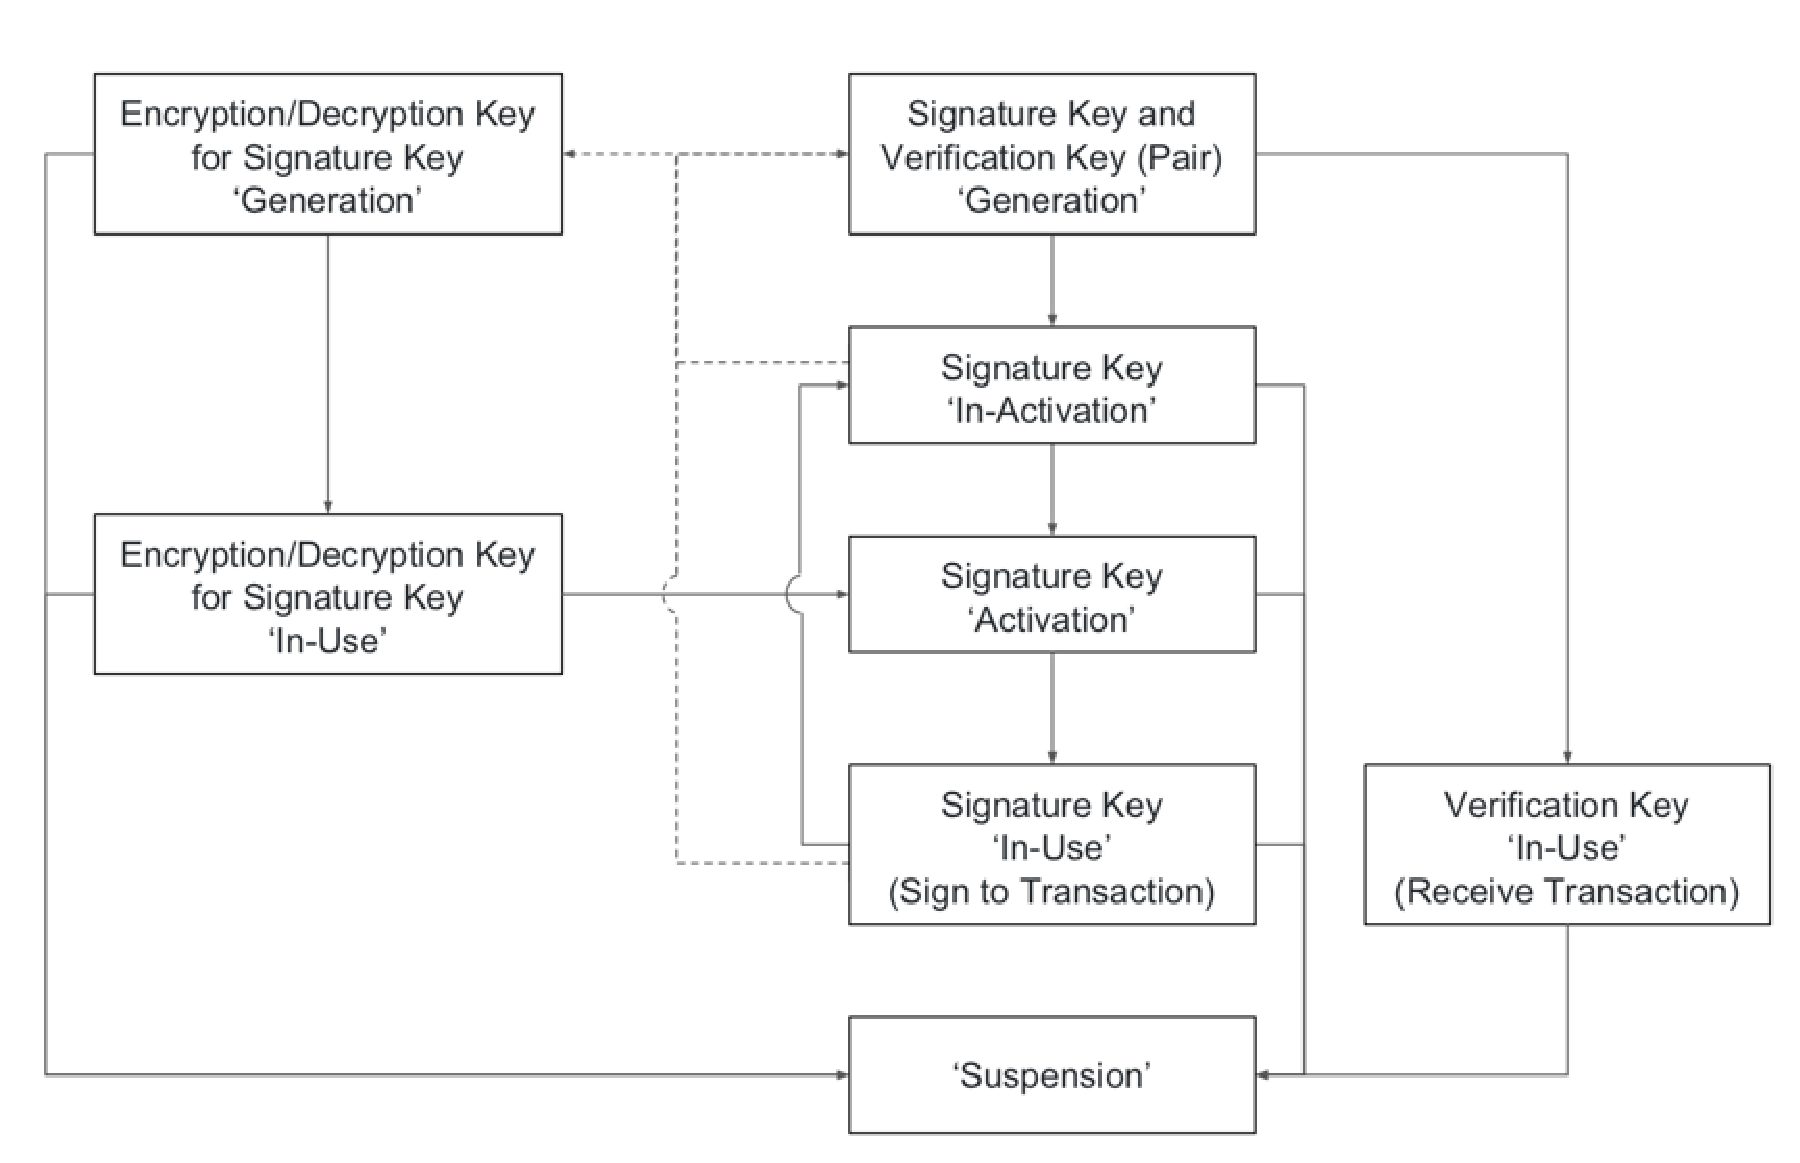
\includegraphics[width=4.5cm,pagebox=cropbox,clip]{key_lifecycle.pdf}
        \caption{Key life-cycle at cryptocurrency exchange}
        \label{key_lifecycle}
      \end{center}
    \end{minipage}
  \end{tabular}
\end{figure}


The model consists of Customer Interface for UI for login and transaction, Customer Authentication Function, Customer Credential Database, Customer Assets Management Function, Blockchain Node for incoming transactions, Incoming transaction management Function, Order processing function, Assets Database, Transaction Singing Function for outgoing transactions, Exchange Operation Modules, Operator Authentication Function and Operator Audit Database. Details are described in Appendix~\ref{appendix_system_model}

We defined each functional element to distinguish functions logically, and do not show the actual arrangement on the actual system.
%For example, in our actual system, address management unit may be managed by an integrated database. Also, there are implementations with multiple functions packaged together. For example, each functional element of the transaction signature system may be integrated with the customer property management system, or the transaction signature system may be operating as another system.

\begin{table}
 \caption{Keys in cryptocurrency exchange}
 \begin{tabular}{ll} \hline
  Types                     & Description                                             \\ \hline
  Signature Key             & A private key for signing transactions                  \\
                            & (asymmetric key cryptography)                           \\ \hline
  Verification Key          & A public key for verification of transactions           \\ % (asymmetric  \\
                            & (asymmetric key cryptography)                           \\ \hline% Recipient address of transactions
  % &  are unique value calculated from verification key) \\ \hline
  Encryption/decryption key & Secret key to keep confidentiality of signature key     \\
  for signature key         & (symmetric key cryptography)                            \\ \hline

  Master Seed               & A seed to generate a signature key in decisional wallet \\ \hline
 \end{tabular}
 \label{tbl_4_1}
\end{table}

After a pair of a signature key and a verification key (hereafter “key pair”) is generated, an address to receive transactions is generated from the verification key. By notifying a sender of crypto assets this address, the sender is able to transfer the asset to the address. When the recipient transfers the asset to the other address, the original recipient signs the transaction data which includes the transfer order. Inactive state of the signature key is the state such that the signature key is stored in confidential manner in the signature key management function of Fig.~\ref{fig_system_model}. An example of inactivation is encryption by encryption/decryption key (e.g. pass phrase), that is, the signature key is encrypted. In contrary, activation is the process to make the key usable to sign, by decrypting the inactivated key. The activation is assumed to be executed in transaction signing function of Fig.~\ref{fig_system_model}. Activation and inactivation may be executed in an implementation of wallet, when the wallet have both functions. The signature key is not needed after its generation until execution of signing to transaction. Thus, there is a way to manage the signature key in offline manner with storing the verification key and address online(cold wallet).

\begin{description}
 \item[On the usage of multiple keys:]
       In some crypto assets system, it is recommended not to use the same key pair twice, thus it produces multiple key pairs. This feature is for preventing trace and not relevant to the business efficiency of a cryptocurrency exchange.
       %However, a cryptocurrency exchange should manage addresses for each customer. Thus it should manage multiple key pairs for the same crypto assets.
 \item[On the suspension of keys:]
       Suspension of key usage is only an operation inside a cryptocurrency exchange. By definition of blockchain based crypto assets system, any user cannot cancel transaction once it is made. As another case, it is difficult to revoke signature key even after the suspension of key. For example, a customer accidentally operate some crypto assets for suspended address. In such case, the suspended signature key is needed to make an reimbursement. Thus, suspension of keys should be conducted with considering such cases.
\end{description}

%In the cryptocurrency exchange, the role and risk of the signing key are extremely large. This is not only to enable the transfer of coins but also to disappear due to the anonymity of the Crypto Asset, the property that it is impossible to revocation the signing key against leakage / theft or roll back the transaction by.
%In this section, we show the risk of fraudulent use that could lead to the loss of the signing key, leakage / theft, and damage of value. It also shows supply chain risk etc. when introducing Wallet related to signature key.

\subsection{Analysis based on security management standard}
%\subsection{Analysis based on governance and security management standard}

%At cryptocurrency exchanges, it is mandatory to establish, conduct, maintain and continuously improve security management. As requirements in term os security management, items described in [ISO.27001:2013] are sufficiently considered according to the business process of each cryptocurrency exchange. Especially, following items should be carefully considered, because a cryptocurrency exchange retains customer’s asset and should deal with issues specific to crypto assets.
\begin{description}
 \item[On stakeholders]\footnote{ISO 27001~\cite{ISO27001} Clause 4}
       It is needed to consider protection of customer’s assets, as well as division of responsibility with outsourcers including security of private key management for crypto asset, and mattes by which a cryptocurrency exchange may give social impacts like money laundering.
 \item[On security policy]\footnote{ISO 27001~\cite{ISO27001} Clause 5}
       A cryptocurrency exchange should define a security policy which includes security objectives and controls. Especially, it is recommended to disclose the security policy on the management of crypto assets to customers to facilitate self evaluation.
 \item[Continuous risk evaluation and improvement]\footnote{ISO 27002~\cite{ISO27002} Clause 6, 8, 9 and 10}
       A cryptocurrency exchange should watch security risks of crypto assets in addition to aligning the general security management framework, because the risks change and increase due to rapid development of related technology. It is especially important to continuously evaluate risk and improve security objectives, policy and controls to keep effectiveness of security controls after starting their operations. A cryptocurrency exchange should decide security objectives and controls with considering viewpoint as countermeasure to threat as lost, theft, leak and abuse of customer’s assets data and private key for crypto assets, requirements for actual business, compliance to laws and rules and social responsibilities to prevent crimes in use of crypto assets like scam and money laundering.
\end{description}
The cryptocurrency exchange conducts threat analysis, vulnerability evaluation, risk evaluation and defining security objectives and controls according to its actual business and system. Security objectives and controls should be decided with considering threats and risks specific to crypto assets, as well as general security objectives and controls described in ISO 27002~\cite{ISO27002}.
%Followings are items of security objectives and controls described in [ISO.27002:2013].
%\begin{itemize}
%  \item Information Security Policies
%  \item Organization of information security
%  \item Human resource security
%  \item Access control
%  \item Cryptography
%  \item Physical and environmental security
%  \item Operations security
%  \item Communications security
%  \item System acquisition, development and maintenance
%  \item Supplier relationships
%  \item Information security incident management
%  \item Information security aspects of business continuity management
%end{itemize}
%Consideration of above items is mandatory. Next close describes specific items to be considered by a cryptocurrency exchange.

\subsubsection{Risk analysis of signing secret key}
Risk analysis differs depending on the assumed threats, system
configuration, threat modeling, and so on.
%In this section, we show
%a case study based on the following assumption as an example.
Here,
the threat concerning the signature secret key and the factors that
can cause the threat are assumed as follows.
%In addition, we assumed
the following as the actor giving input to the signing secret key
based on Fig.~\ref{fig_system_model}% in \ref{Threat modeling and security requirements}.

\begin{itemize}
 \item Threats: lost, leakage, theft and fraudulent use.
       %  \begin{itemize}
       %    \item lost
       %    \item leakage, theft
       %    \item fraudulent use
       %  \end{itemize}
 \item Factors of Threats: mis-operations, legitimate users' malice, spoofing, intrusions from outside and unintended behaviors of implementations.
       %    \begin{itemize}
       %    \item mis-operations
       %    \item Legitimate users' malice
       %    \item Spoofing
       %    \item Intrusions from outside
       %    \item Unintended behaviors of implementations
       %    \end{itemize}
 \item Actors: exchange operation modules, transaction signing modules, customer asset management function implementation and incoming coin management function implementation.
       %  \begin{itemize}
       %     \item exchange operation modules
       %     \item Transaction Signing modules
       %     \item customer asset management function implementation
       %     \item incoming coin management function implementation
       %  \end{itemize}
\end{itemize}

% move to appendix
%  Factors of threats are organized as follows.
%
%  Mis-operation: An act that an authorized user (including an
%  administrator) of the system accidentally operated by mistake.  For
%  example, it is incorrectly supposed that an operation to coin 100,000
%  yen is incorrectly dispatched for 1 million yen.

%  Legitimate users' malice: Acts performed by a legitimate user of the
%  example, theft or unauthorized use of the signature private key due
%  to internal fraud.  In this case, it is the purpose of identifying
%  acts that can be factors, and the purpose and incentive of the act
%  are not limited here.

%  Spoofing: An act other than an authorized user of the system
%  impersonating a legitimate user (more accurately impersonating some
%  kind of operation).  For example, an internal burglar without
%  administrator privilege accesses the system with administrator
%  authority.

%  Intrusions from outside: an act of an outsider accessing the system
%  malicious intrusion from the outside by exploiting the system's
%  vulnerability, incorporating malware into the exchanging system via
%  targeted e-mail to the exchanges' administrator or the like and
%  generating a private signature private key (or transaction creation)
%  from the outside, Allow remote control of etc.

%  Unintended behaviors of implementations: The system behaves
%  unexpectedly by the designer or operator irrespective of the
%  intention or malice of the operation.  For example, a signature
%  private key leaks due to a bug in the exchange management system.

Of these threat factors, theft and fraudulent use are regarded as
threats that can only be caused by explicit malicious factors.
% As a
% result, the possible risks for signing key to be assumed are the
% figured in appendix \ref{appendix_risks}


%Objectives of security management at a cryptocurrency exchange contain secure protection of customer’s asset, compliance to business requirements, laws and rules, and realization of social responsibility. Security policies and execution statements derived from such objectives are recommended to be publicly available for consumers, business partners, auditor and regulators to help their judge.

%\section{Directions and action items to secure cryptocurrency exchanges}
\section{Directions to secure cryptocurrency exchanges}
\subsection{Required technologies}
From above analysis, there are six issues where we need to consider to introduce enhanced technologies to make cryptocurrency exchange trustable.
\begin{description}
 \item[Authenticity and integrity of segregated ledger:]
       Many cryptocurrency exchanges manage customers' assets by using the segregated ledger, and
       they record not all transactions on the public blockchain, because of efficiency and latency
       reasons. Assuring integrity and authenticity of segregated ledger is essential part of
       security of their business. Introducing transparent way,
       such as cryptographic timestamp, to assure such characteristics is needed.

 \item[Muti-signature:]
       Multi-signature is a major technology to avoid loss of customers' asset when loss of one or
       minor part of keys occurs.

 \item[Underlying cryptography and implementation:]
       HSM is the trust anchor of cryptocurrency exchange. In general, HSM supports standard cryptographic
       algorithms. However, cryptocurrency may implement special algorithm or parameter as curve of ECC.
       Standardization of underlying cryptography and selecting HSM which supports
       more algorithms are needed.

 \item[Kay management and wallet:]
       Most cryptocurrency exchanges manage assets using hot wallet for online transaction and cold wallet
       to protect keys from attack from network. For online wallet, utilizing certification program like
       FIPS 140-2 or CMVP and products with such certification is needed.

 \item[Audit:] Internal audit and third party audit is needed to provide transparency to customers
       and regulators. Technology to make such audit easy such as cryptographic time stamp is needed.

 \item[External evaluation:]
       To clarify the security level of implementation, certification as common criteria (ISO/IEC 15048)
       is needed. Establishing protection profile is helpful to conduct external evaluation.
\end{description}

\subsection{Required operations}

\begin{description}
 \item[Basics of key management]
       %In general, followings are required in management of private cryptographic keys.
       In general private cryptographic keys.
       % They
       should be isolated from other informational assets, the number of access to private keys should be limited as minimum as possible and be prepared for unintentional lost of private keys.
       %\begin{itemize}
       %\item They should be Isolated from other informational assets. Rigorous access control is mandatory.
       %\item Limit the number of access to private keys as minimum as possible.
       %\item Be prepared for unintentional lost of private keys.
       %\end{itemize}
       %Followings are three basic security control to realize above. Additional security controls specific to crypto assets custodians are described in and after sub-clause {{security-controls-at-crypto-assets-custodian}}.
       Three security controls as State management of private keys, Administrator role separation and mutual check-and-balance and Backup of private key are needed.

       %\begin{enumerate}
       %  \item State management of private keys \\
       %As described in \ref{key_lifecycle}, a private key has one of multiple states, and it may be active or inactive state in its operation. The private key should be in active state when it is used for signing or decryption. It is recommended to enforce to input some secret information to activate an inactive private key. This makes keep the inactive private key away from abuse, if the adversary does not have the secret information. This method ensure security of the private key against leakage and lost.\\
       %It is also recommended to minimize the term of activation to limit the risk of abuse as minimum as possible. Unnecessary activation of secret key increases the risk of abuse, leakage and theft, though keeping the activation state is efficient from business viewpoint. On the other hand, frequent activation/inactivation may give impact to business efficiency. It is important to consider the trade-off between the risk and business efficiency and provide clear key management policy to customers.
       %  \item Administrator role separation and mutual check-and-balance\\
       %It is fundamental form of operation of a critical business process which uses private key to perform cryptographic operations by multiple party to prevent internal frauds and errors. For example, by setting isolated rights on digitally signing and approval to go into the area of signing operation, it becomes difficult for single adversary to give an malicious digital signature without known by the third party. Additionally, the enforcement of attendance of other person is effective security control to internal frauds and mis-operations.
       %  \item Backup of private key\\
       %Lost of private key makes signing operations by using the key impossible any more. Thus backup of private key is an important security control. On the other hand, risks of leakage and theft of backup keys should be considered. It is needed to inactivate the backup key.
       %\end{enumerate}

 \item[Backup]

       Backup is the most fundamental and effective measure against lost of signing key. On the other hand, there are  risks of leakage and lost of backup device. These risks depend on the kind backup device, thus security controls on such devices should be considered independently.
       %Followings describe typical backup devices and leakage/theft risks associated with them.
       Typical ways are Cloning to tamper-resistant cryptographic key management device, Backup to storage for digital data and Backup to paper.

       %\begin{itemize}
       %  \item Cloning to tamper-resistant cryptographic key management device \\
       %  If a signing key is managed by a tamper-resistant key management device (device X) and X has cloning function, cloning the key to another device Y is the most secure way to backup the key, where the cloning function is the technique to copy the key with keeping confidentiality to other devices than X and Y. The implementation of the function is recommended to be evaluated/certified by certification program like CMVP or FIPS 140. Note that, the cryptographic algorithms supported by such tamper-resistant key management devices are limited and all crypto assets systems can utilize it, but it is one of the most secure way of backup.
       %  \item Backup to storage for digital data \\
       %  Here, it is assumed to backup keys to storage like USB memory and DVD. There are two types of operations; one is backup data is stored in movable devices in offline manner, the other is backup data is stored in online accessible manner. If the device is movable, the possibility of steal and lost increases, thus the device should be kept in a cabinet or a vault with key, and the access control to such cabinet/vault should be restrict. \\
       %  Of the backup storage is online, risks of leakage and theft should be assumed as same as the key management function implementation inside the crypto assets custodian. In general, the same security control is recommended to such backup storage. If there is some additional operation, for example the backup device is inactivated except for the time of restore, the security control may be modified with considering operation environment. When it is not avoided the raw key data is be outside of the key management function implementation, the custodian should deal with the problem of remained magnetics.
       %  \item Backup to paper\\
       %  There is a way to backup keys in offline manner, to print them to papers as a QR code or other machine readable ways. It is movable than storage for digital data and easy to identify. There remains some risk of leakage and theft by taking a photo by smartphone and so on.
       %\end{itemize}

 \item[Offline management]
       There is a type of offline key management (as known as "cold wallet") which isolates private keys from the system network to prevent leakage and theft caused by intrusion.

       %In this case, some offline operation is needed to make the system use the key. Examples are, keys are usually stored inside a vault and connected to the system only when it is utilized, and USB memory is used to data transportation between an online system and an offline system.  If there is not explicit approval process in the offline operation for key usage, anyone cannot stop malicious transaction. That is, this solution can prevent lost and theft, however, an explicit approval process is needed to prevent abuse of keys.

 \item[Distributed management]
       It is also a good security control to distribute the right to use private key to multiple entity. There are two examples; division of secret key and multi-signature.
\end{description}

%\begin{itemize}
%\item Division of secret key\\
%Division of the signing key to multiple parts, then manage them by multiple isolated system is an effective measure to protect the keys against leakage and theft. This document does not recommend  a specific technique, but recommends to implement this control based on a certain level of security evaluation like secret sharing scheme. In that case, secure coding and mounting penetration test are needed to eliminate the implementation vulnerabilities. This method is also effective to backup devices.
%\item Multi-Signature\\
%This is a signature scheme which requires multiple isolated signing keys to sign a message. It is effective to protect each key hold by an entity and signing mechanisms. There are many different realization of multi-signature and they are different according to specific crypto assets system. Thus, consideration on preparing multiple implementations and their interoperation is need when a crypto assets custodian operate multiple crypto assets.
%\end{itemize}

%\paragraph{Other issues}
%
%In this sub-clause, following topics will be described.
%
%\begin{itemize}
%  \item Security of wallet implementation
%  \item Monitoring of private key access
%  \item Log audit
%\end{itemize}

% \subsection{Fixing pitfalls}
% One of the sources of problems is gaps in understandings among stakeholders. There are four major stakeholders; cryptocurrency exchange, cryptocurrency engineers/researchers, regulators, and customers.
% Cryptocurrency exchange might start the business without sufficient knowledge of security management,
% and assumptions in operating cryptocurrency system, though any technology has an assumption and limitation for
% operation.
% As a result of the investigation, most cryptocurrency exchanges do not have qualified knowledge
% and capability to operate as financial institutions. Some exchange does not deal with requests from the regulatory authority, that is, there might not be a common language for communication between
% cryptocurrency exchanges and regulators.
% Regulators also do not have enough technical knowledge to evaluate the technological reliability of each
% cryptocurrency.
% Customers need the knowledge to evaluate each cryptocurrency and transparency for the operation of
% cryptocurrency exchange. However, currently, disclosure by cryptocurrency exchange is not sufficient.
% Many scams occur from this asymmetry of knowledge.
% Such a difference of understandings is a source of difficulties to solve the problem.
% We need to create a common dictionary for conversation among all stakeholders and
% a neutral place to communicate in a multi-stakeholder manner.

\subsection{Toward standardization}

%As described in section 1, it is too early to define some technology and operational standards at well-recognized standardization body like ISO, IEC, ITU-T, etc, because blockchain technology and its architecture is currently dynamically changing.
%However,
Though it is too early to define some technology and operational standards,
some standardization bodies started already their activities and study toward the future standard.
On the security of cryptocurrency exchange, ISO TC307 started two projects to make a technical report on the security of blockchain and distributed ledger technology (ISO TR23245) and a technical report on security practice of digital asset custodians (ISO TR23576).
%Here, ``digital asset custodians'' means financial institutes which store digital assets and/or credentials (cryptographic keys, etc. ) associated with the digital assets, hence existing cryptocurrency exchanges are included in this category of institutes.
% The study described in section 4 is now developed as an internet draft in IETF.
%The almost same contents are described in ISO TR23576.
%Despite the difficulty to create a technical standard on blockchain technology,
% Such standard or agreed document is needed to operate any organization
% associated with blockchain technology, because they store and utilize cryptographic keys. These documents are useful not only for constructing
% a cryptocurrency exchange, but also audit, creating and operating management lifecycle, providing pieces of evidence of secure operation to the public, and
% earning trust to operators of trustless financial systems.

\section{Conclusion}
% Giving the unfortunate occurences of huge incidents at cryptocurrency exchanges, Japan is the most advanced country to deal with cryptocurrency governance issues. In spite of the advanced regulation on the exchanges in Japan, investigations by JFSA after the incidents reveal the shortage of technical, operational, and governance expertise.
The analysis implies the needs of a feedback loop for continuous enhancement. We conducted modeling and risk analysis on the cryptocurrency exchange, aligning to ISO/IEC 27000, and created an example system and key management model. We found that the key lifecycle and management model is largely different from ordinary PKI. We showed typical key management model from the analysis. Establishing a concrete loop and new key management especially for PoS, is essential to not re-invent the wheel and to make a healthy cryptocurrency ecosystem.


\begin{thebibliography}{21}
\bibitem{N08} Satoshi Nakamoto, ``Bitcoin: A Peer-to-Peer Electronic Cash System,'' \textit{https://bitcoin.org/bitcoin.pdf}.

% \bibitem{IETF18}
% M. Sato, M. Shimaoka, and H. Nakajima, ``  General Security Considerations for Crypto Assets Custodians,''
%  \textit{https://tools.ietf.org/html/draft-vcgtf-crypto-assets-security-considerations-02}

% \bibitem{ISOTR23576}
% S. Matsuo and A. L. Castro (ed.), ``ISO TR 23576: Blockchain and distributed ledger technologies -- Security of digital asset custodians,''  under development,
% \textit{https://www.iso.org/standard/76072.html}

\bibitem{FSAGUIDELINE}
Japanese Financial Services Agency, ``Guidelines for Administrative Processes: Financial Companies No16,''
\textit{https://www.fsa.go.jp/policy/virtual\_currency/02.pdf}

\bibitem{FSAREPORT}
Japanese Financial Services Agency, ``Interim report of inspection and monitoring on cryptocurrency exchanges,''
\textit{https://www.fsa.go.jp/news/30/virtual\_currency/20180810-2.pdf}

\bibitem{MUFG}
MUFG, ``Annual Report (USGAAP),''\\
\textit{https://www.mufg.jp/english/ir/annualreport/2018mufg/pdf/mar/ar2018.pdf}

\bibitem{ISO27001}
``ISO/IEC 27001:2013: Information technology — Security techniques — Information security management systems — Requirements,''  \\
\textit{https://www.iso.org/standard/54534.html}

\bibitem{ISO27002}
``ISO/IEC 27002:2013: Information technology -- Security techniques -- Code of practice for information security controls,''  \\
\textit{https://www.iso.org/standard/54533.html}

\end{thebibliography}

\begin{subappendices}
%\renewcommand{\thesection}{\appendixname~\Alph{section}}
\section{Other concrete examples of issues showed in the JFSA's report}
\label{appendix_report_examples}

The following is the other examples of issues showed in the JFSA's interim report from investigation and monitoring that are not discussed in section 2.

\begin{enumerate}
  \item First line: Issues around advertisements
   \begin{itemize}
     \item An exchange does not have the internal review process of the contents of the advertisement.
     \item An exchange used TV advertisement on which famous celebrity calls the name of the certain cryptocurrency to encourage customers to buy it while explains risks only in few seconds.
     \item An advertisement shows a particular discount period and investment profitability that customers cannot verify.
   \end{itemize}

  \item Second line: Issues around AML/CFT
  \begin{itemize}
    \item Many exchanges fail to confirm customers' characteristics and purpose of the transaction as well as conduct pre-examination to exclude transactions with the organized crime group.
    \item There are cases of lack of appropriate guidelines regarding checking process of impersonation
    \item An exchange lacks monitoring process and system to detect suspicious activities.
  \end{itemize}

  \item Second line: Issues around segregation of customers' assets
  \begin{itemize}
    \item Several exchanges fail to reconcile between bank account balance for customers' assets and account balance on their own server.
    \item An exchange fails to find out the cause of the frequent incident that the customers' bank account balance becomes below the balance on their own server.
    \item Several exchanges create general ledger only and fail to keep books on daily transactions, the ledger of their own account, and the ledger of customers' account, all of which are required by regulation.
  \end{itemize}

  \item Second line: Issues around system safety management
  \begin{itemize}
    \item Several exchanges neither keep records of system troubles that keep date/time and the number of incidents, impact, countermeasures, and changes to prevent re-emergence nor understand the root cause of the system troubles even though they had many troubles.
    \item In the system development phase, an exchange neither establishes documents for requirement definition, development plan, and architecture specification nor conducts implementation tests at the frontline.
  \end{itemize}

  \item Second line: Issues around customer protection
  \begin{itemize}
    \item When an exchange issues its own currency, it fails to explain the financial situation and business model of the issuing exchange to customers.
    \item Another exchange issuing new currency fails to disclose important information that management of the exchange gain a huge bonus for sale of the cryptocurrency.
    \item Several exchanges fail to conduct a training program on customers' information management and allow anyone in the company and third-party contractor to access to it or even bring out from the company.
    \item Several exchanges fail to either keep records of the customer complains or improve the business practice based on the complaints. They just ignore them or randomly address them case by case basis.
  \end{itemize}

  \item Third line: Issues around internal audit
  \begin{itemize}
    \item Many exchanges fail to establish a plan for internal audit.
    \item Even when an internal audit was conducted, several exchanges fail to do it based on the risk assessment.
    \item Several also fail to conduct the audit on the third party contractor.
  \end{itemize}

  \item Corporate culture and governance
  \begin{itemize}
    \item Within many exchanges, board meeting fails to discuss how to mitigate risks associated with their business as financial institutions.
    \item Many exchanges fail to disclose their business and financial situation to customers in an easy-to-understand manner, which other financial institutions are required.
  \end{itemize}

\end{enumerate}

\section{Details of system model}
\label{appendix_system_model}
\begin{itemize}
 \item Customer Interface\\
       Provides screen and input functions such as login process, account management (deposit/withdrawal instruction etc.) and trade instruction for the customers(users). Web application, API, etc.
 \item Customer Authentication Function\\
       Performs user authentication process for login to the cryptocurrency exchange.
 \item Customer Credential Database\\
       Manages required IDs for login and verification information related to user authentication process (f.g password verification info.).
 \item Customer Assets Management Function\\
       A group of functions to manage customer accounts. Receive instructions for deposit or withdrawal (outgoing coins) and perform processing according to the user instructions. Refer or update asset data.
 \item Blockchain Node\\
       Connects to another blockchain nodes to retrieve blockchain data.
 \item Incoming transaction management Function\\
       Checks transaction stored in blockchain and confirm whether incoming coins are involved in the specified addresses.
 \item Order processing function\\
       A group of functions that receives sales instructions from customers and performs processing related to trading of crypto assets. Refers and updates asset data based on asset data.
 \item Assets Database\\
       Manages holdings of fiat currencies and crypto assets. It does not include the private keys for signing transactions. Managed separately from the assets of the excahnge for each customer.
 \item Transaction Singing Function, which includes Transaction Generator, Transaction Broadcaster, Transaction Signing Function, Address Management,
       \begin{itemize}
        \item Transaction Generator\\
              Generates transactions to be sent to the blockchain based on instructions from the customer asset management system or the exchange management system, and Private Signature Key Management Function
        \item Transaction Broadcaster\\
              Sends the signed transaction to the blockchain. Connects to nodes of the another nodes on the blockchain.
        \item Transaction Signing Function\\
              Generates digital signatures based on the instructed transaction contents and the private signature key (with IDs and addresses).
        \item Address Management\\
              Manages public keys with related to the private signature keys, or addresses (such as values calculated from the public keys).
        \item Private Signature Key Management Function\\
              Manages the signing keys of the crypto assets (the keys used for the transaction signing). Sometimes it is separated into the cold-wallet as security countermeasure. “Signature key generator” creates signature keys. The generated keys are registered in the signature key management unit, and the public keys and addresses are registered in the address management units.
       \end{itemize}
 \item Exchange Operation Modules\\
       A group of functions for exchanges’ administrators. Based on operations from administrators, instructs generation of generating new signature keys or transfer crypto assets.
 \item Operator Authentication Function\\
       Authenticates the administrator users.
 \item Operator Audit Database\\
       Manages verification data related to the authentication processes of the administrators.
\end{itemize}

\section{Risk analysis}
\label{appendix_risks}

The following list shows the result of risk analysis on the
model of cryptocurrency exchange.

\begin{enumerate}
  \item Threat by lost - Risk of Unauthorized operation (with legitimate
         path)
   \begin{itemize}
     \item End-user's malice
     \item Operator's malice in Custodian
     \item Spoofing to end users
     \item internal frauds (spoofing to operators) - Risk of Intrusion from the outside
     \item Intrusion into the transaction signing modules
     \item Intrusion into the incoming coin management function (implementation)
     \item Intrusion into the customer asset management function (implementation)
     \item Intrusion into the exchange operation modules - Risk of System Behaviors different from human operation
     \item Unintended behaviors of the transaction signing modules
     \item Unintended behaviors of the incoming coin management function (implementation)
     \item Unintended behaviors of the customer asset management function (implementation)
     \item Unintended behaviors of the exchange operation modules - Risk of mis-operation (by human error)
     \item Mis-operation of end user
     \item Mis-operation of operator
   \end{itemize}

  \item Threat by leakage - Risk of Unauthorized operation (with legitimate path)
  \begin{itemize}
    \item End-user's malice
    \item Operator's malice in Custodian
    \item Spoofing to end users
    \item internal frauds (spoofing to operators) - Risk of Intrusion from the outside
    \item Intrusion into the transaction signing modules
    \item Intrusion into the incoming coin management function (implementation)
    \item Intrusion into the customer asset management function (implementation)
    \item Intrusion into the exchange operation modules - Risk of System Behaviors different from human operation
    \item Unintended behaviors of the transaction signing modules
    \item Unintended behaviors of the incoming coin management function (implementation)
    \item Unintended behaviors of the customer asset management function (implementation)
    \item Unintended behaviors of the exchange operation modules - Risk of mis-operation (by human error)
    \item Mis-operation of end user
    \item Mis-operation of operator
  \end{itemize}
  \item Threat by theft - Risk of Unauthorized operation (with legitimate path)
  \begin{itemize}
    \item End-user's malice

    \item Operator's malice in Custodian

    \item Spoofing to end users

    \item internal frauds (spoofing to operators) - Risk of Intrusion from the outside

    \item Intrusion into the transaction signing modules

    \item Intrusion into the incoming coin management function (implementation)

    \item Intrusion into the customer asset management function (implementation)

    \item Intrusion into the exchange operation modules
  \end{itemize}
  \item Threat by fraudulent use - Risk of Unauthorized operation (with legitimate path)
  \begin{itemize}
    \item End-user's malice
    \item Operator's malice in Custodian
    \item Spoofing to end users
    \item internal frauds (spoofing to operators) - Risk of Intrusion from the outside
    \item Intrusion into the transaction signing modules
    \item Intrusion into the incoming coin management function (implementation)
    \item Intrusion into the customer asset management function (implementation)
    \item Intrusion into the exchange operation modules
  \end{itemize}
\end{enumerate}

\end{subappendices}

\end{document}
